\documentclass[UTF8,12pt,a4paper]{ctexart}
\usepackage[a4paper,margin=2.3cm]{geometry}
\usepackage{amsmath,amssymb}
\usepackage{graphicx}
\usepackage{tabularx}
\usepackage{array}
\usepackage{longtable}
\usepackage{hyperref}
\usepackage{float}
\graphicspath{{figures/}}
\hypersetup{colorlinks=true,linkcolor=blue,urlcolor=blue,citecolor=black}
\setCJKmainfont{SimSun}
\setlength{\parindent}{2em}
\setlength{\parskip}{0.35em}
\emergencystretch=1em
\renewcommand{\arraystretch}{1.25}
\newcommand{\toprule}{\hline}
\newcommand{\midrule}{\hline}
\newcommand{\bottomrule}{\hline}
\newcommand{\hashblockcn}{%
\begin{center}
\begingroup\ttfamily\small
24128AAD2EE45EEA7E6B63EBBD9992CD\\
F25D0483A2CEBEFBFC13BC69079AF1F2
\endgroup
\end{center}}
\title{切分协议对公开液压试验台可报告性能的影响：\\蓄能器等级识别与名义压力误差审计}
\author{严晨宇}
\date{2026年10月}
\pagestyle{plain}
\begin{document}
\maketitle

\section*{摘要}
\textbf{目的：}评估数据切分协议如何改变公开液压试验台上蓄能器压力等级识别的报告结果，并比较离散等级表示与数值回归在名义压力误差上的差异。

\textbf{方法：}使用 UCI Machine Learning Repository 的 Condition Monitoring of Hydraulic Systems 数据集。数据包含 2205 个 60 s 循环和 17 路信号；从六个压力通道和一个电机功率通道提取每循环 70 个统计特征。以蓄能器四个名义压力等级（90、100、115、130 bar）为主任务，比较循环随机、profile 连续块、已观测四部件组合留出（state4-OC）和含 stable 标志的五标签组合（state5）四种外层协议。嵌套分组交叉验证使用五个划分种子；模型在每个外层训练集内按平衡准确率选择。另在相同 state4-OC 外层折上进行固定模型和分类—回归配对审计。

\textbf{结果：}五种子中，随机循环与 state4-OC 的 pooled OOF 平衡准确率中位数分别为 0.983（0.981–0.985）和 0.870（0.860–0.875）。在同一 state4-OC OOF 循环上，分类预测映射到名义压力后的 MAE 为 1.83 bar，数值回归为 7.74 bar。权重审计显示，分类循环等权、state4 组合等权和 profile 块等权 accuracy 分别为 0.884、0.876 和 0.866；回归 MAE 分别为 7.74、5.35 和 5.39 bar。

\textbf{结论：}在本数据和建模流程下，切分协议改变了蓄能器分类的点估计及其对应的估计对象；观察到的差异属于完整评估流程，不能单独解释为泄漏因果量。四个名义压力等级支持离散状态识别评价，不支持连续压力测量或跨设备外推。本文的价值在于把协议、估计对象和误差表示放在同一可复核评价框架中。

\textbf{关键词：}液压系统；状态监测；交叉验证；分组评估；蓄能器压力；有序误差

\section*{English Abstract}
\sloppy
\textbf{Objective:} To evaluate how data-splitting protocols change reported accumulator pressure-level identification on a public hydraulic test rig, and to compare discrete target representation with numeric regression for nominal-pressure error.

\textbf{Methods:} We used the UCI Condition Monitoring of Hydraulic Systems dataset, which contains 2,205 60-s cycles and 17 signal channels. Seventy cycle-level summary features were extracted from six pressure channels and one motor-power channel. The main task was classification of four nominal accumulator pressure levels (90, 100, 115, and 130~bar). Four outer protocols were compared: random cycles, profile-contiguous blocks, observed four-component combination holdout (state4-OC), and five-label combinations including the stable flag (state5). Nested grouped cross-validation used five split seeds, with model selection inside each outer training set. Fixed-model and paired classification--regression audits used the same state4-OC outer folds.

\textbf{Results:} Across five seeds, median pooled OOF balanced accuracy was 0.983 (0.981--0.985) for random cycles and 0.870 (0.860--0.875) for state4-OC. On the same state4-OC OOF cycles, MAE after mapping classification labels to nominal pressure values was 1.83~bar, compared with 7.74~bar for numeric regression. The weighting audit gave classification accuracies of 0.884, 0.876, and 0.866 for cycle, state4-combination, and profile-block weighting, respectively; regression MAE was 7.74, 5.35, and 5.39~bar.

\textbf{Conclusion:} In this dataset and workflow, the split protocol changes both the point estimate and the estimand. The differences are properties of the full evaluation workflow, not an identified causal leakage amount. The four nominal levels support a discrete state-identification evaluation and provide no evidence for continuous-pressure or cross-device performance. The contribution is a reproducible evaluation that links split protocol, estimand, and error representation.

\textbf{Keywords:} hydraulic system; condition monitoring; cross-validation; grouped evaluation; accumulator pressure; ordinal error

\section{引言}
液压状态监测的结果不仅取决于特征和分类器，也取决于数据如何被切分。本文使用 UCI Machine Learning Repository 的 Condition Monitoring of Hydraulic Systems 数据集；官方页面记录一套液压试验台的多速率信号和组件状态 profile，共 2205 个实例、17 个信号文件，数据 DOI 为 10.24432/C5CW21，许可为 CC BY 4.0[1]。已有研究从多元统计、传感器故障补偿和周期特征提取等角度处理该类监测任务[2–4]，国内研究则提供了多元件识别、多传感器健康评估和深度模型诊断的任务参照[11–14]。

同一数据集已经出现多组件分类和传感器归因研究[5,6]。战欣和刘卓娅[15]进一步报告了基于 144 个状态组合的高测试准确率，但其训练/测试比例、划分单位和归一化拟合范围未完整给出。另一篇 2026 年预印本采用块不相交评估和联合 conformal 预测[7]。这些工作说明该数据集能够产生较高的分类分数，也提示分数必须与切分单位、目标定义和不确定性报告一起解释。本文的切入点是评价协议：不同协议究竟对应什么估计对象，以及离散压力等级和数值回归是否给出相同的误差判断。

重复循环来自同一试验台时，循环随机划分回答的是在相似已观测工况下识别新循环的问题；profile 连续块或状态组合留出则改变了被留出的结构。交叉验证研究也指出，划分应与目标预测情景匹配[9]。因此，本文不把不同协议的分数当作同一性能参数的简单高低，而是把它们作为不同评价情景下的报告结果。

本文回答两个问题：在固定周期统计特征和候选模型搜索流程下，循环、profile 连续块和组件状态组合划分如何改变蓄能器等级分类的点估计；在相同 state4-OC 留出循环上，离散分类与数值回归呈现怎样的名义压力误差。研究贡献是建立可复核的协议—估计对象对应关系，并把多种子 OOF、权重审计和同循环误差比较放入同一评价框架。五种子、固定模型和配对误差分析均属于审查后补充分析。

\section{材料与方法}
\subsection{数据来源与结构审计}
研究使用 UCI 官方发布的 Condition Monitoring of Hydraulic Systems 数据压缩包[1]。本地归档压缩包 SHA-256 为：\hashblockcn。数据包括 2205 个连续编号的 60 s 循环、17 路信号文件和一个逐循环五列 profile。六个压力信号 PS1–PS6 与电机功率 EPS1 的采样率为 100 Hz，每循环 6000 点；流量信号 FS1、FS2 为 10 Hz，每循环 600 点；温度 TS1–TS4、振动 VS1、CE、CP 和 SE 为 1 Hz，每循环 60 点。

本地审计逐行检查 17 个信号文件的行数、采样点数、空行、解析错误、非有限数值和 profile 对齐。各文件均有 2205 个循环，采样点数与官方说明一致，未发现空行、解析错误或非有限值。该审计回答文件结构和数值可解析性；传感器校准、测量偏差和实验批次独立性属于外部验证问题。

profile 前四列分别给出冷却器、阀、泵内泄漏及蓄能器状态，末列为 stable 标志。冷却器具有 3、20、100 三个标记水平；阀具有 73、80、90、100 四个水平；泵内泄漏具有 0、1、2 三个等级；蓄能器标签为 90、100、115、130 bar。stable=0 对应达到稳定条件，stable=1 表示静态条件可能尚未达到；本文将其作为条件标志而非第五种故障类别。CE 和 CP 在数据文档中标作 virtual 信号，SE 的定义为 efficiency factor；本文没有据此推断三者各自对应独立实体传感器[1]。

\subsection{分析任务与单位}
主任务是蓄能器四级状态分类。补充任务是泵内泄漏三级状态分类。原始分析单位为一个完整 60 s 循环，2205 个循环不被视为 2205 个独立实验。为避免把该分组误读为正式时间或批次留出，本文将相邻 profile 五列状态完全相同的连续循环称为“profile 连续块”，共 194 块，其中 36 块长度为 1 个循环、154 块长度为 10 个循环、1 块长度为 19 个循环、2 块长度为 200 个循环、1 块长度为 210 个循环。忽略 stable 后有 144 个不同四部件状态组合；包含 stable 后有 180 个不同五列状态向量。profile 连续块和状态组合均由公开 profile 推导，并非官方批次或设备编号。

为避免将该协议误读为设备或批次验证，本文将由 profile 前四列（cooler、valve、pump\_leak、accumulator）组成的精确状态组合留出记为“已观测四部件组合留出”，英文简称 \texttt{state4-OC}（OC 表示 observed-combination）。这里的“未见”只指训练折中未出现的组合编码；同一试验台、同一公开记录中的压力等级仍会在其他组合中出现。该名称不表示未知设备、未知蓄能器等级、独立采集批次或工业现场验证；原始脚本和结果文件中的 \texttt{state4} 标签仅作为实现标识保留。

\subsection{特征构造}
主分类使用 \texttt{pressure\_power} 通道组，即 PS1–PS6 和 EPS1，共七个 100 Hz 测量通道。对每个信号的每个循环计算均值、总体标准差（ddof=0）、最小值、最大值、极差、10\%分位数、中位数、90\%分位数、末点减首点以及相邻样本绝对差的平均值。分位数由 NumPy 的 \texttt{quantile} 默认线性插值计算。七路信号各提取 10 个特征，共 70 个。本文将末点减首点作为差分特征，将相邻样本绝对差均值作为变化量特征，不把二者解释为物理斜率或变化率。特征按每个 60 s 周期独立提取；周期之间的先后关系仅用于构造 profile 连续块和状态分组，不作为模型输入。

\subsection{分类器与嵌套模型选择}
分类候选模型为逻辑回归、径向基核支持向量机（RBF-SVM）和随机森林。逻辑回归与 SVM 使用训练折内拟合的 \texttt{StandardScaler}；随机森林不进行标准化。每个外层训练折内按平衡准确率选择候选模型及参数。搜索空间为：逻辑回归 $C\in\{0.1, 1, 10\}$，最大迭代数 2500；RBF-SVM $C\in\{1, 10\}$，\texttt{gamma="scale"}；随机森林树数 300、\texttt{max\_features="sqrt"}。分类共六个候选配置。相同候选网格用于各划分协议。

主结果采用外层 5 折、内层 3 折嵌套交叉验证，以降低在候选模型选择后直接报告同一交叉验证误差所带来的选择偏差[10]。每个外层测试折只由其余折训练数据完成模型选择和拟合。分类的外层和内层分组均采用 \texttt{StratifiedGroupKFold}，设置 \texttt{shuffle=True}；对种子 s 的内层第 k 个外层折使用种子 s+k。随机协议将每个循环赋予唯一 group，因此保持类别分层但允许相近循环分散到训练和测试集。其他协议按预先定义的 profile 连续块、state4-OC 或 state5 组号进行分组。

五种子分析使用 \texttt{20261013} 至 \texttt{20261017}。原始主结果为种子 20261013；其余四种子在检查主结果后加入，用于划分敏感性和稳健性检查，不作为预注册重复实验。分类器自身如随机森林固定 \texttt{random\_state=20261013}，从而种子变化反映交叉验证划分改变，不另行改变随机森林内部随机种子。软件环境为 Python 3.14.3、NumPy 2.4.4、SciPy 1.17.1 和 scikit-learn 1.9.1。

这五个种子不是五个独立实验，也不是从目标总体抽取的重复样本；其范围只描述同一 2205 个物理循环重新分配折时的结果变化。由于新增四种子是在检查 20261013 结果后才决定，仍存在分析选择风险；重复运行同一批循环不能消除该风险，因此这些结果不能解释为独立稳健性确认、置信区间或显著性证据。

另在种子 20261013 的相同外层折上拟合三种固定配置（逻辑回归 C=10、RBF-SVM C=10、随机森林 300 棵树），不进行内层选择。该分析用于区分模型选择变化与固定模型下观察到的协议差异；它在查看嵌套主结果之后追加，属于探索性对照。

\subsection{数值回归比较}
辅助数值回归以 90、100、115、130 作为数值响应，候选模型为 Ridge（$\alpha\in\{0.1, 1, 10, 100\}$）、RBF-SVR（$C\in\{1, 10, 100\}$、\texttt{gamma="scale"}、epsilon=0.1）和随机森林回归（300 棵树、\texttt{max\_features="sqrt"}）。线性模型与 SVR 使用训练折内标准化；回归候选模型依据内层平均 MAE 选择，外层及内层均使用同一 state4-OC 分层分组折法。数值预测不施加 90–130 bar 边界。

为提供直接可读的等级基线，将分类器 OOF 类别预测固定映射为各自名义压力值（90、100、115 或 130 bar），并与数值回归在同一 cycle ID、真实标签和外层折上配对。该映射是依据现有分类 OOF 的事后派生比较，分类器按平衡准确率选择，并未按压力 MAE 调优。另在每个外层折内，以训练集的多数压力等级构造多数类基线，以训练集平均压力构造均值回归基线；二者均不使用测试折特征或标签。数据标签是四个离散设定值而非独立测得的连续压力真值；分类映射的 bar 误差表达相对名义等级的偏差；连续压力测量能力需要连续参考值和独立采集批次验证。

\subsection{补充分析}
补充泵内泄漏分类沿用主分析的 \texttt{pressure\_power} 特征、state4-OC 分组、种子 20261013、外层 5 折/内层 3 折嵌套模型选择流程、候选模型及平衡准确率选择准则。该分析是对同一数据集另一组件标签的探索性复核。

蓄能器通道组敏感性分析在相同 state4-OC 划分和种子下比较五组统计特征：\texttt{all} 包含 17 路信号（170 个特征）；\texttt{physical} 包含除 CE、CP、SE 外的 14 路信号（140 个特征）；\texttt{low\_rate} 包含 TS1–TS4、VS1、CE、CP、SE 共 8 路信号（80 个特征）；\texttt{pressure\_flow} 包含 PS1–PS6、FS1、FS2 共 8 路信号（80 个特征）；\texttt{pressure\_power} 包含 PS1–PS6、EPS1 共 7 路信号（70 个特征）。每组使用相同嵌套模型选择流程。该比较只评估现有通道组合的预测结果，不代表硬件配置、传感器成本或部署收益。

stable 分层结果从主任务完整的 state4-OC OOF 预测中按 profile 的 stable 值分层计算，不在各层内重新拟合模型。共同支持描述限定于同时包含 stable=0 和 stable=1 循环的 state4-OC 组合，并报告相应循环数和蓄能器标签构成；不进行组合等权的配对效应估计。这些分层结果作为条件描述；由于样本量和等级构成不同，不作 stable 条件的因果效应估计。

\subsection{划分协议及估计目标}
四种划分协议定义如下。

\begin{table}[H]
\centering
\small
\begin{tabularx}{\linewidth}{>{\raggedright\arraybackslash}X >{\raggedright\arraybackslash}X >{\raggedright\arraybackslash}X >{\raggedright\arraybackslash}X}
\toprule
协议 & 分组单位 & 主要测试情景 & 已知限制 \\
\midrule
random & 单个循环 & 从同一记录总体随机留出循环 & 相邻或重复工况可跨训练/测试集 \\
profile 连续块 & 相邻且五列 profile 完全相同的连续块 & 每个测试折留出若干由 profile 推导的连续恒定状态块 & 长短块高度不均，时间相邻块仍可分属训练/测试集；不等同于正式批次留出 \\
state4-OC & cooler、valve、pump\_leak、accumulator 的精确组合 & 测试训练中未出现的四部件组合，但压力等级在其他组合中已出现 & 不是未知压力等级、设备、批次或现场测试 \\
state5 & 上述四部件状态与 stable 标志的精确组合 & 留出已观测的五列状态组合 & 不能保证相邻组合或相关时间段隔离 \\
\bottomrule
\end{tabularx}
\end{table}
为把指标解释绑定到可由公开 profile 近似的评价情景，本文采用如下决策表。这里的“部署目标”只是公开 profile 能近似表达的评价情景，不是对真实设备部署的验证。

\begin{table}[H]
\centering
\small
\begin{tabularx}{\linewidth}{>{\raggedright\arraybackslash}X >{\raggedright\arraybackslash}X >{\raggedright\arraybackslash}X >{\raggedright\arraybackslash}X}
\toprule
可近似的评价目标 & 候选评价协议 & 估计对象 & 当前数据不能支持的外推 \\
\midrule
同一试验台、已观测状态下识别新循环 & random & 循环级点预测 & 未知设备、批次或时间段泛化 \\
同一试验台、识别未见的已观测四部件组合 & state4-OC & 组件组合留出下的循环级点预测 & 未知蓄能器压力等级、独立设备或工业现场 \\
按相邻相同 profile 段落留出 & profile 连续块 & profile 推导块留出下的点预测 & 正式时间批次、采集日期或因果时间效应 \\
区分已观测 stable 条件组合 & state5 & 五标签组合留出下的点预测 & stable 条件的因果效应或设备独立性 \\
\bottomrule
\end{tabularx}
\end{table}
冷却器标签具有时间顺序结构；数据没有可用的设备编号、独立采集日期或正式实验批次标识。因此，各分组按已观测状态结构阻止特定单位跨折；跨折样本的统计独立性仍需设备或批次标识验证。四种协议同时改变训练/测试样本组成、可共享状态信息和模型选择环境，其差异是不同评估流程所得估计之差，不是对数据泄漏量或切分协议因果效应的识别。

\subsection{评价指标与汇总}
主分类结果报告准确率、平衡准确率、宏 F1 和混淆矩阵。准确率按循环等权计算；平衡准确率为各类别召回率的算术平均，宏 F1 为各类别 F1 的算术平均。pooled OOF 指标先合并各外层测试折的循环级预测，再按各指标定义计算，因此平衡准确率与宏 F1 是在循环级 OOF 汇总上对类别等权平均。组级多数投票准确率先在每组内分别取真实标签和预测标签的众数，再按组等权汇总。

有序误差按四个等级在 [90,100,115,130] 中的索引计算，报告精确等级准确率、一阶邻域命中率（索引距离$\leq 1$，包含完全命中）、平均等级距离，以及距离为 0、1、2、3 的计数。数值回归另报告原始 bar 预测的 MAE、RMSE 和 R²。除循环池化指标外，本文先在每个 state4-OC 组合或 profile 连续块内计算循环损失，再对组合或块等权平均；另按四个真实压力等级等权汇总 MAE。组合等权和块等权是不同估计对象，不是独立设备或批次的置信区间。五种划分种子计算 pooled OOF 指标的中位数、范围和均值/标准差，正文表格展示中位数和范围；这些范围描述五次对同一数据集重新分配折的变化，不代表总体置信区间。没有对折或种子进行显著性检验，因为折间训练集重叠且同一批物理循环在多种子重复中反复使用。

\section{结果}
\subsection{数据与组结构}
结构审计确认 2205 个循环与 17 路信号文件完整对齐。蓄能器标签分布为 90、100、115、130 bar 各 808、399、399、599 个循环；stable=0 与 stable=1 分别为 1449 和 756 个循环。分组登记得到 194 个 profile 连续块和 144 个四部件状态组合。块长度分布明显不均，两个 200 循环块、一个 210 循环块和一个 19 个循环块占据长段结构；因此 profile 连续块留出仍受到有限大块数和时间排序的限制。

\subsection{嵌套模型选择下的协议敏感性}
表1汇总五种划分种子的 pooled OOF 平衡准确率与宏 F1；五种子中位数和范围是本文的主估计，原始单种子只作为参考。随机循环划分在五个种子中均高于 state4-OC；但 profile 连续块、state4-OC 与 state5 之间的顺序并不稳定。随机划分平衡准确率中位数为 0.983，state4-OC 为 0.870；两者取值范围分别为 0.981–0.985 和 0.860–0.875。逐种子配对的 random−state4-OC 平衡准确率差值中位数为 0.111（0.107–0.124），宏 F1 差值中位数为 0.116（0.110–0.124），准确率差值中位数为 0.100（0.093–0.105）。这些差值只描述同一批循环在不同折分下的变化，不进行显著性检验。原始单种子 20261013 的四协议平衡准确率为 random 0.981、profile 连续块 0.882、state4-OC 0.870、state5 0.875；对应宏 F1 为 0.982、0.880、0.866、0.872。追加的四个种子是在检查原始结果后加入，不能解释为独立稳健性确认、总体置信区间或显著性证据。

\begin{table}[H]
\centering
\small
\begin{tabularx}{\linewidth}{>{\raggedright\arraybackslash}X >{\raggedright\arraybackslash}X >{\raggedright\arraybackslash}X}
\toprule
协议 & 平衡准确率中位数（五种子范围） & 宏 F1 中位数（五种子范围） \\
\midrule
随机循环 & 0.983（0.981–0.985） & 0.982（0.981–0.985） \\
profile 连续块 & 0.880（0.873–0.887） & 0.878（0.872–0.885） \\
state4-OC 四部件组合 & 0.870（0.860–0.875） & 0.866（0.859–0.872） \\
state5 五标签组合 & 0.876（0.871–0.891） & 0.872（0.868–0.889） \\
\bottomrule
\end{tabularx}
\end{table}
五种子中随机与 state4-OC 的平衡准确率范围不重叠；该结果描述同一组物理循环在不同划分下的稳定性，不构成独立重复试验或显著性检验。循环随机划分的较高分与跨折存在相同或相近工况信息的可能性相符，但现有设计不能把差值单独归因为信息泄漏。

除等级等权的平衡准确率外，本文对循环、组合和 profile 块三种权重进行了敏感性审计。循环等权分类 accuracy 为 0.884；state4-OC 组合内先平均再对 144 个组合等权的 accuracy 为 0.876；profile 连续块内先平均再对 194 个块等权的 accuracy 为 0.866。数值回归 MAE 分别为 7.741、5.346 和 5.390 bar；四个压力等级等权 MAE 为 6.850 bar。回归误差随权重变化明显，说明 7.741 bar 只代表循环池化估计，不能被解释为典型组合或典型 profile 块的误差。完整每折分布和单位明细见 \texttt{results/weighted\_metrics\_audit\_20261016.json}。

\subsection{固定模型下的协议比较}
固定分类器补充结果显示，不同分类器的协议间分数变化幅度不同（表2）。随机划分下，随机森林平衡准确率为 0.981；profile 连续块、state4-OC、state5 下分别为 0.760、0.744、0.766。RBF-SVM 在随机划分为 0.920，在三种分组协议约为 0.720–0.736。逻辑回归的随机划分结果为 0.930，三种分组结果则在 0.870–0.882。主嵌套搜索中随机协议各折均选择随机森林，state4-OC 各折均选择 C=10 的逻辑回归，因而主分析随机与 state4-OC 的差值同时包含模型选择改变。固定模型对照说明模型敏感性并非均匀，不能把主分析差值解释为与分类器无关的纯切分效应。

\begin{table}[H]
\centering
\small
\begin{tabularx}{\linewidth}{>{\raggedright\arraybackslash}X >{\raggedright\arraybackslash}X >{\raggedright\arraybackslash}X >{\raggedright\arraybackslash}X >{\raggedright\arraybackslash}X}
\toprule
固定模型 & 随机 & profile 连续块 & state4-OC & state5 \\
\midrule
逻辑回归，C=10 & 0.930 & 0.882 & 0.870 & 0.875 \\
RBF-SVM，C=10 & 0.920 & 0.736 & 0.720 & 0.729 \\
随机森林，300棵树 & 0.981 & 0.760 & 0.744 & 0.766 \\
\bottomrule
\end{tabularx}
\end{table}
表2为原始种子 20261013 下的 pooled OOF 平衡准确率，属于探索性参考。固定模型对照是在查看主结果后补做，协议间仍有测试组成和训练/测试依赖结构差异。

\begin{figure}[H]
\centering
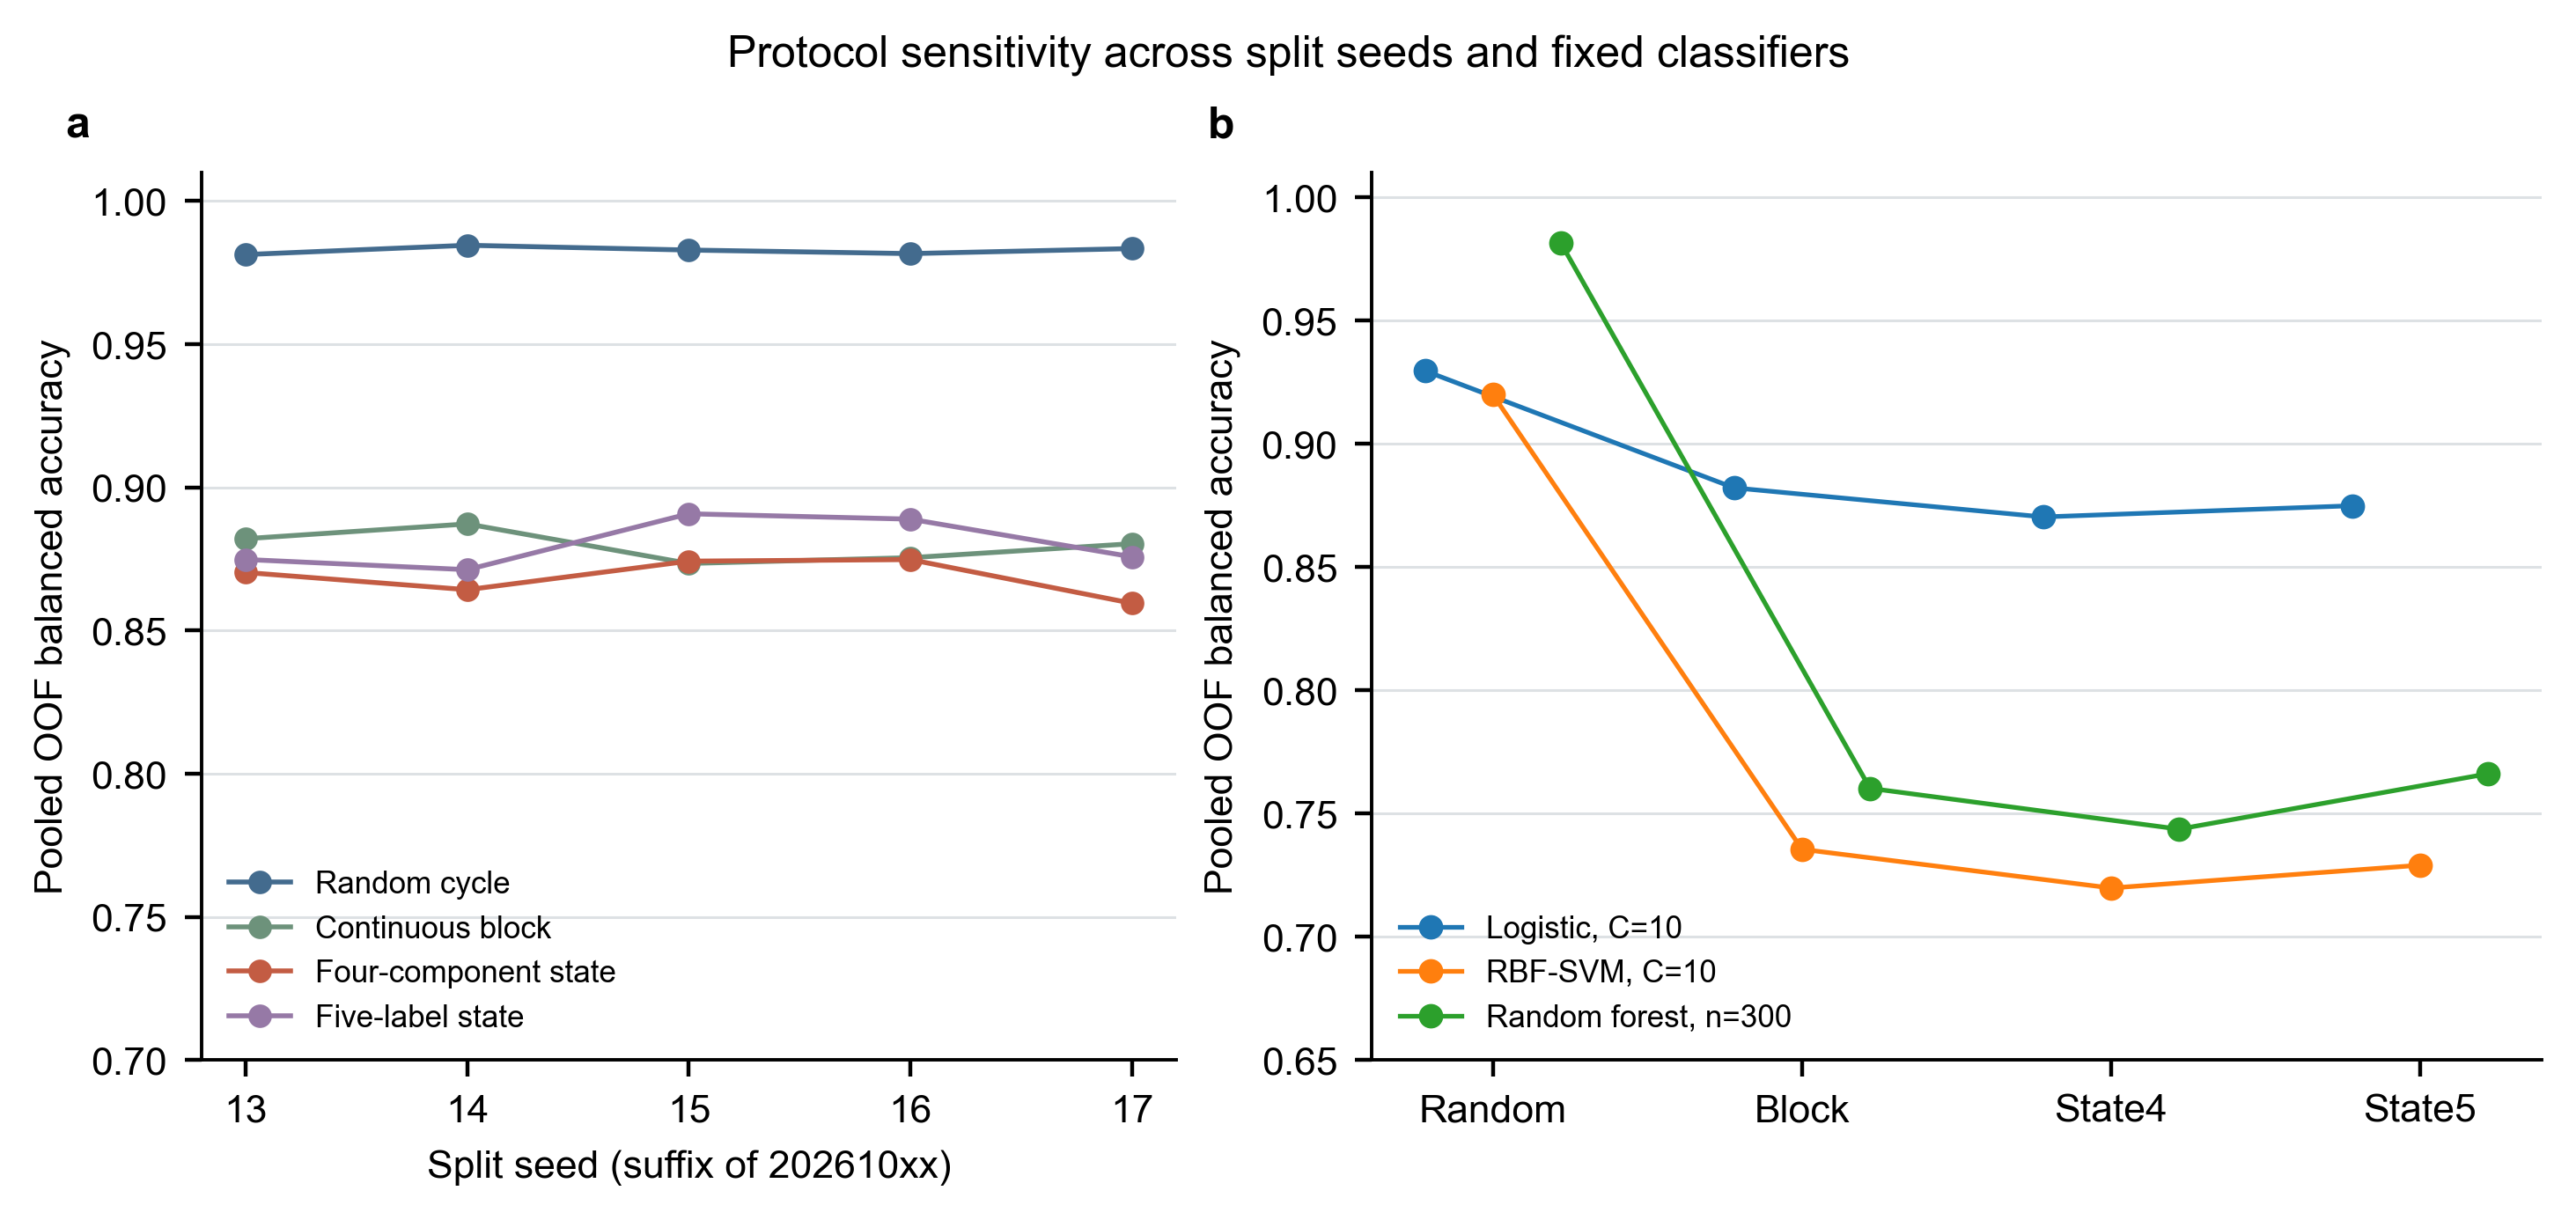
\includegraphics[width=0.94\linewidth]{figures/hydraulic_protocol_robustness_20261013.png}
\caption{图1：蓄能器分类协议敏感性与固定分类器比较}
\label{fig:1-1}
\end{figure}

\subsection{蓄能器主协议分类结果}
在 \texttt{pressure\_power}、state4-OC 及原始单种子 20261013 的参考运行中，蓄能器 pooled OOF 平衡准确率为 0.870，宏 F1 为 0.866，准确率为 0.884；按 144 个四部件组合多数投票的组级准确率为 0.938。五折均选择逻辑回归 C=10。循环级混淆矩阵见表3。五种子中位数 0.870 和范围 0.860–0.875 已在表1作为主估计报告。

\begin{table}[H]
\centering
\small
\begin{tabularx}{\linewidth}{>{\raggedright\arraybackslash}X >{\raggedright\arraybackslash}X >{\raggedright\arraybackslash}X >{\raggedright\arraybackslash}X >{\raggedright\arraybackslash}X}
\toprule
真实\textbackslash{}预测（bar） & 90 & 100 & 115 & 130 \\
\midrule
90 & 758 & 30 & 15 & 5 \\
100 & 21 & 334 & 44 & 0 \\
115 & 1 & 37 & 329 & 32 \\
130 & 4 & 4 & 63 & 528 \\
\bottomrule
\end{tabularx}
\end{table}
256 个分类错误中，227 个为相邻等级错分，29 个跨越至少两个等级索引。90 bar 类的 50 个错误中，20 个被分到 115 或 130 bar。错误因此以相邻等级为主，但仍包括非相邻混淆。

\subsection{离散分类与数值回归的配对误差}
在同一 state4-OC OOF 循环上的事后描述性配对中，分类器预测等级映射到名义 bar 数值后，按 2205 个相同循环计算得到 MAE 1.83 bar、RMSE 5.74 bar、R² 0.878、精确等级准确率 0.884、一阶邻域命中率 0.987、平均等级距离 0.133。数值回归原始输出的对应 MAE 为 7.74 bar、RMSE 为 11.85 bar、R² 为 0.480、最近等级准确率为 0.689、一阶邻域命中率为 0.906、平均等级距离为 0.446。两套 OOF 的 cycle ID、真实标签和外层折逐项一致。

数值回归输出有 352/2205（16.0\%）低于 90 bar 或高于 130 bar，预测范围为 64.82–198.50 bar。按最近等级映射后的距离为 0、1、2、3 的循环数分别为 1519、478、119、89；208 个至少跨越两级的错误中，200 个来自第二外层折。该折占样本数的 21.6\%，却贡献 41.7\% 的绝对误差和 65.2\% 的平方误差；该折 MAE 为 14.94 bar、R² 为 -0.731，并选择 RBF-SVR（C=100）。该模型内层平均 MAE 为 5.68 bar，但外层折表现明显较差。越界预测和严重等级误差是两种不同诊断：前者有 352 个，后者集中于第二折；逐循环交叉表显示两者没有重合样本，因此不能把它们合并为一个“主要错误类型”。本研究没有预先定义或统计检验一个可排序的“主要错误类型”。该折诊断提示折间失配风险，不能通过删除该折来替代完整 OOF 汇总，也不能确定失配由单一模型或特定工况造成。进一步的只读构成检查显示，第二折包含一个 200 循环的长块（block 64），占该折 476 个循环的 42.0\%；该块对应 profile $20\_100\_0\_90$、stable=1 和真实 90 bar，块内回归 MAE 为 31.10 bar，预测均值为 121.10 bar。该定位支持“折组成与不均衡块大小可能造成敏感性”的解释，同时保留特征分布和模型失配等替代解释。

为减少输出空间和目标函数差异造成的误读，公平审计在完全相同的 state4-OC 外层折、70 个特征和训练折内标准化条件下，增加了限幅回归、有序累积阈值分类、多数/均值基线和固定模型族对照。原始回归 MAE 为 7.741 bar，限幅到 90–130 bar 后为 6.666 bar；简单有序控制 MAE 为 2.433 bar、平衡准确率为 0.830；分类映射 MAE 为 1.828 bar。多数类基线的准确率为 0.366、平衡准确率为 0.250、映射 MAE 为 17.200 bar；均值基线的 MAE 为 15.394 bar、RMSE 为 16.696 bar、$R^2$ 为 -0.032。固定线性族中，分类映射 MAE 为 1.828 bar，回归限幅 MAE 为 5.018 bar。该结果支持的表述是当前四个离散名义等级任务中的协议内描述性差异，不支持分类算法普遍优于回归或连续压力测量能力。完整定义和逐折结果见公平比较审计记录。

\begin{figure}[H]
\centering
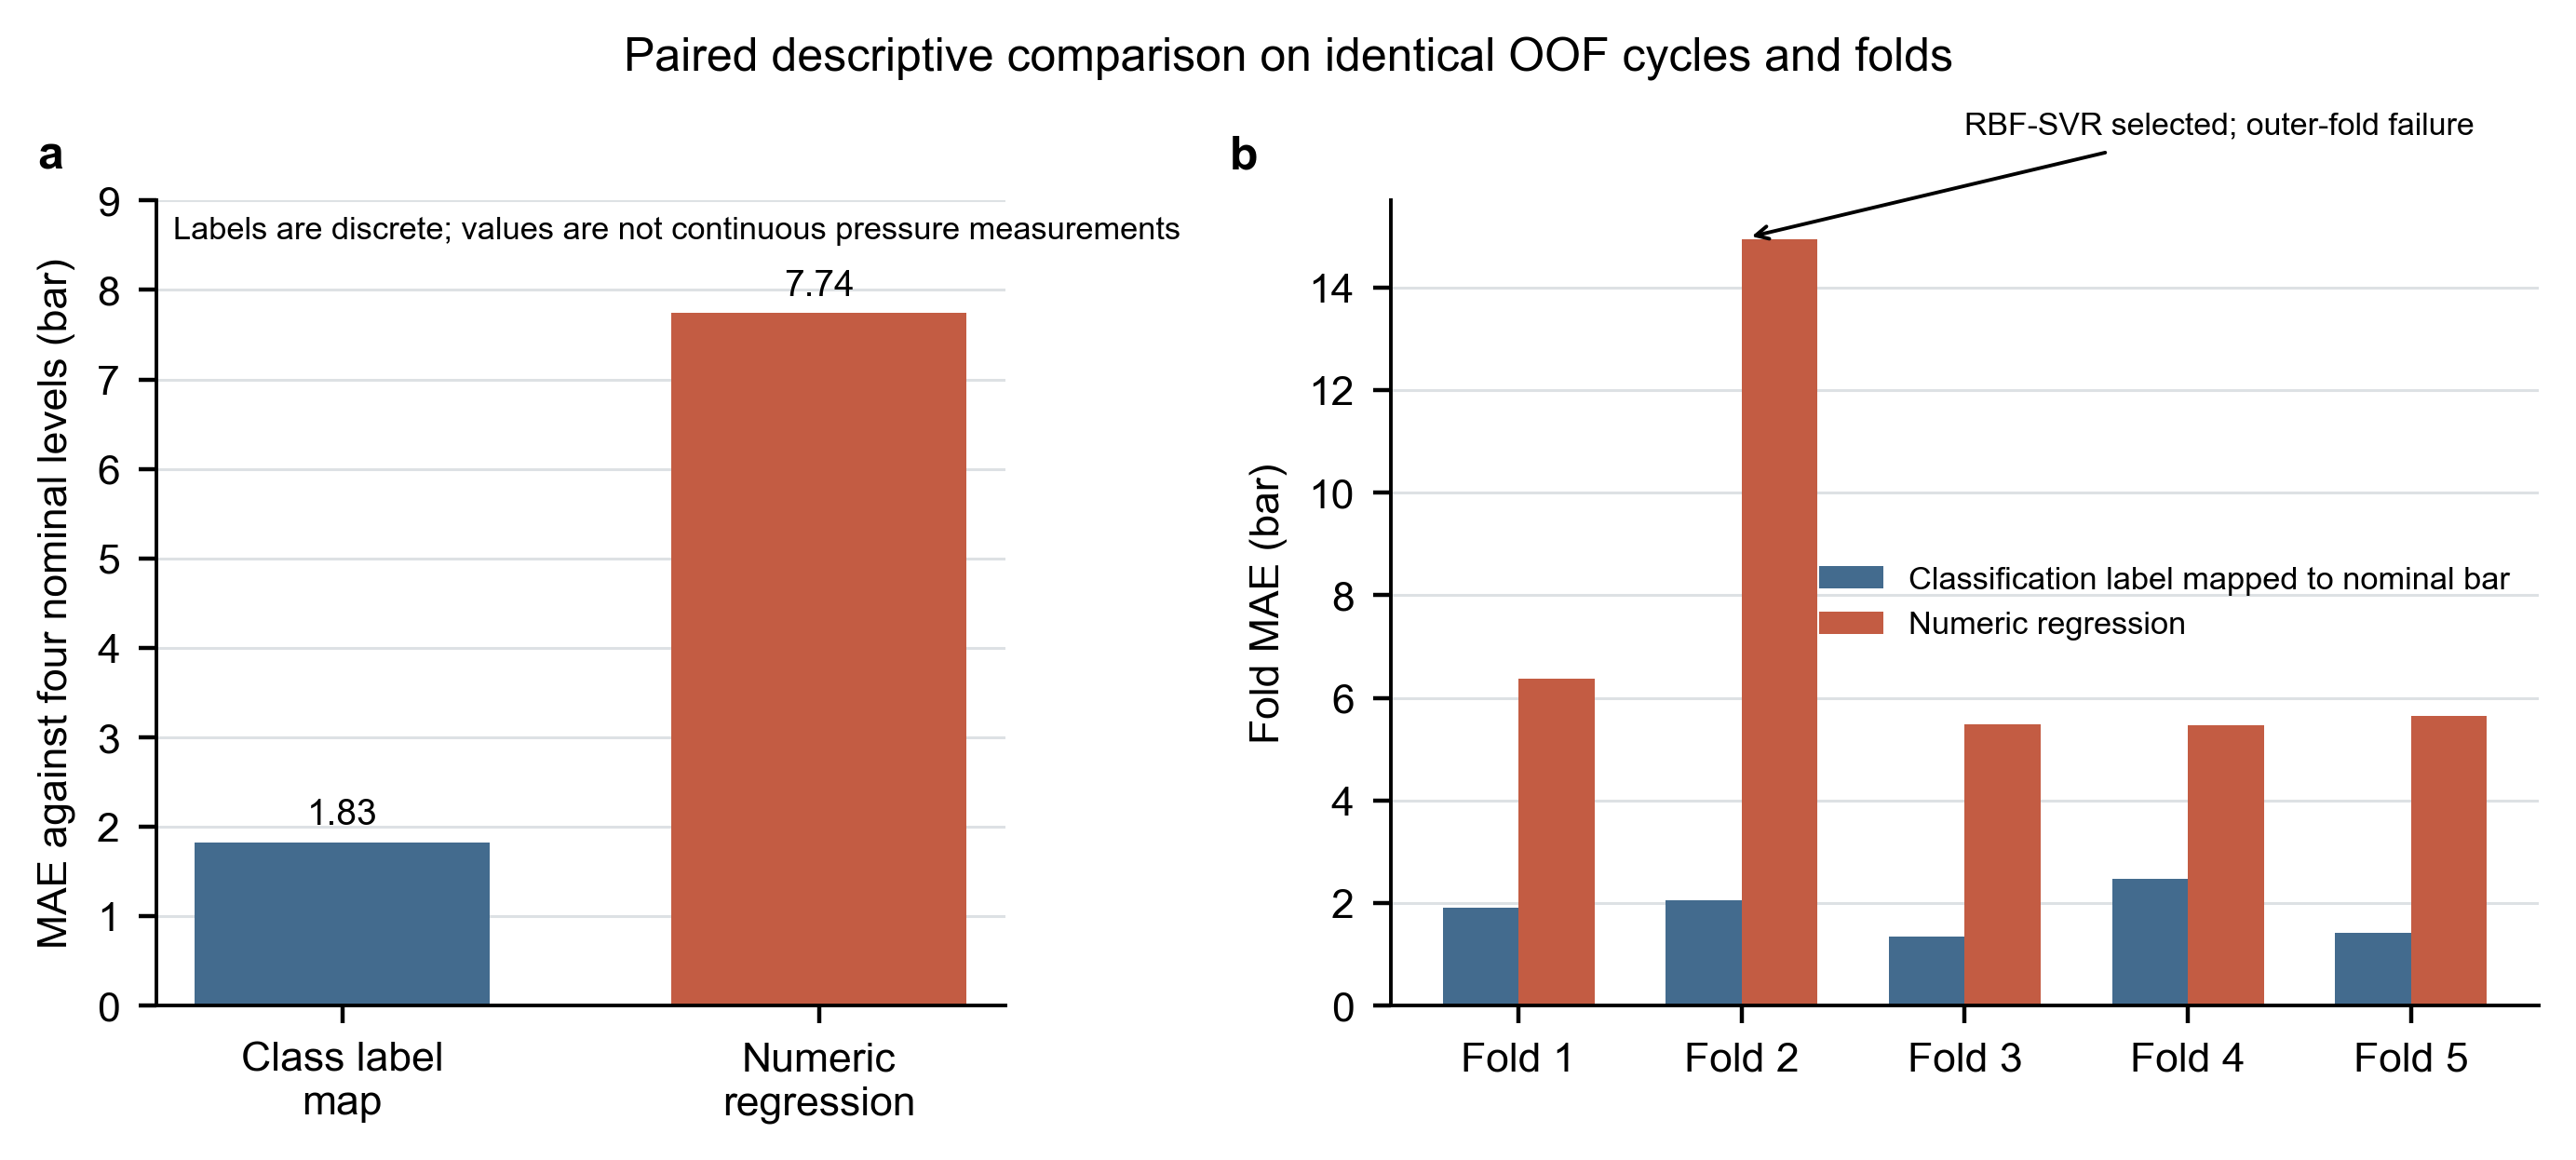
\includegraphics[width=0.94\linewidth]{figures/hydraulic_estimator_comparison_20261013.png}
\caption{图2：分类名义压力误差与数值回归误差比较}
\label{fig:2-2}
\end{figure}

分类映射结果更好不等于分类器能够测出任意连续压力：标签只有四个设定等级，分类模型按平衡准确率优化，映射值没有级间连续分辨率。该对照只说明在现有离散标签任务中，连续回归没有带来更低的等级或名义压力误差。数值回归被保留为辅助分析，以展示原始回归输出和折间不稳定性。

\subsection{次要分类与条件分层}
为检验把目标标签放入 state4-OC 分组键所带来的解释限制，本文另做 \texttt{context3 = cooler × valve × pump\_leak} 补充分组。固定逻辑回归 C=10、训练折内标准化、seed=20261013 下，36 个 context3 组合完全与训练折隔离且每个测试组合保留四个蓄能器等级；pooled balanced accuracy 为 0.894，context 等权 balanced accuracy 为 0.892，最低 context balanced accuracy 为 0.675。该补充分析仍使用同一试验台、同一公开记录，且配置在查看初始结果后确定，不能替代独立设备或批次验证；它只说明不含目标标签的工况组合留出可以作为更直接的敏感性对照。

泵内泄漏 state4-OC 补充分类在原始单种子下 pooled OOF 平衡准确率为 0.985、宏 F1 为 0.983。该结果用于单一试验台已观测状态组合的补充描述。原始单种子 20261013 下，五个预设信号组在蓄能器 state4-OC 任务的平衡准确率依次为：\texttt{pressure\_flow} 0.878、\texttt{pressure\_power} 0.870、\texttt{all} 0.835、\texttt{physical} 0.820、\texttt{low\_rate} 0.803。\texttt{physical} 是排除 CE、CP、SE 后的 14 通道代理组。该排序仅为探索性描述；现有组间结果没有实测布设、校准、同步、维护或 BOM 费用，不作为稳健的通道组优劣或硬件成本最优性证据，也不构成新传感器选择算法。

同一完整主 OOF 表按 stable 标志分层时，蓄能器 stable=0（1449 个循环）平衡准确率为 0.881、宏 F1 为 0.881；stable=1（756 个循环）分别为 0.819 和 0.748。stable=1 的蓄能器等级数为 439/39/39/239（90/100/115/130 bar）。36 个同时含两种 stable 值的 state4-OC 组合内，stable=0 有 369 个循环，等级数为 99/90/90/90；stable=1 有 756 个循环，等级数仍为 439/39/39/239。这里的 756 个 stable=1 循环与全体 stable=1 层是同一批循环，而不是重新抽取的共同支持子样本。共同支持循环中 stable=0 的平衡准确率为 0.856，stable=1 为 0.819，差值为 0.037，较全层差值缩小约 40%。两层样本量及等级构成不同，且没有按状态组合配对等权的估计；这些值作为条件描述，不作 stable 状态因果效应估计。泵内泄漏总体、stable=0、stable=1 的平衡准确率分别为 0.985、0.988、0.967。

36 个同时含两种 stable 值的 state4-OC 组合内，stable=1 的 756 个循环与全体 stable=1 层是同一批循环，而不是重新抽取的共同支持子样本；因此该分层比较仍应按样本量和等级构成不同的条件描述理解。

\section{讨论}
\subsection{评估协议改变了估计对象}
五种子结果显示，随机循环划分的点估计高于 state4-OC；权重审计还表明，按循环、状态组合和 profile 块汇总会得到不同的总体量。协议同时改变测试样本组成、训练—测试之间共享的工况信息和模型选择环境，因此 random 与 state4-OC 的差异应理解为完整评估流程的差异。该模式与相似循环跨折时随机评估更容易获得较高分数相一致，但数据不能把差异分解为一个独立的泄漏因果量。

state4-OC 阻止完全相同的四部件组合跨外层折，同时保留不同组合中的压力等级，因此它近似对应“已观测压力等级在未见已观测组合上的识别”。profile 连续块和 state5 则分别对应由 profile 推导的相邻段落和含 stable 标志的组合结构；这些单位都不是设备或批次编号。评价时应先定义部署或预测单位，再选择匹配的分组方式。

\subsection{离散目标表示决定压力误差的解释}
蓄能器标签只有四个名义压力设定值。将分类标签映射为名义压力，回答的是离散等级错分造成的压力误差；数值回归则允许级间输出，并承担连续数值误差的解释责任。当前配对结果表明，在这一离散任务和 state4-OC 流程下，分类映射的名义压力误差低于回归；这不是连续压力测量算法之间的普遍优劣判断。若要研究连续压力预测，需要连续参考测量、更多设定值和独立采集批次。

\subsection{与既有工作的关系及评价增量}
本文与同一 UCI 数据上的多组件分类、传感器归因和块级 conformal 研究共享数据背景，但问题不同：本文登记并比较四类切分协议，采用嵌套模型选择和多种子 OOF，并将离散等级误差、回归越界和权重敏感性放在同一审计框架中。战欣和刘卓娅[15]的高准确率结果保留为评价动机，而不作为同目标基准；预印本[7]覆盖了部分分组问题，其主要方法还提供 blockwise joint conformal 覆盖率保证，而本文不提供 conformal 区间或覆盖率保证，也未复刻其数值结果，因此本文将贡献限定为数据集层面的评价补充。对该直接近邻工作的报告透明度判断有明确页级依据：其第 2 页描述数据处理和任务构造，但没有给出可复核的训练/测试比例、划分单位、随机种子或测试集构成；第 4 页图 3 的参数框标为 20 个粒子、30 次迭代，而正文使用相反表述。这里讨论的是报告信息的可复核性，不据此断言其结果无效。

\subsection{局限与应用含义}
证据边界有三点：所有结果来自一套公开试验台，缺少独立设备、采集批次和校准标识；五种子复用同一批循环，且在查看初始结果后追加，属于敏感性描述而非独立确认；主分析使用固定统计特征和有限候选模型，通道组结果也不含硬件成本或部署数据。由此，本文可支持的是数据集级报告建议：报告协议及其估计对象，按需要同时给出循环等权、组等权和离散等级误差。独立设备或批次验证仍需带有相应标识的外部数据。

\section{结论}
在公开液压试验台数据上，切分协议改变了蓄能器分类的点估计及其所对应的估计对象：五种子中随机循环的 pooled OOF 平衡准确率为 0.981–0.985，state4-OC 为 0.860–0.875；分类循环等权、state4 组合等权和 profile 块等权 accuracy 分别为 0.884、0.876 和 0.866；同三种权重下的回归 MAE 分别为 7.74、5.35 和 5.39 bar。差异属于完整评估流程，不能单独解释为泄漏因果量。

四个名义压力等级支持离散状态识别和名义等级误差审计，不提供连续压力或跨设备性能证据。本文的有限增量是把协议、估计对象、权重方式和误差表示置于同一可复核框架中，为公开液压数据的应用评价提供可重复的报告结构。

\section*{数据与研究声明}
\textbf{数据可用性：}原始数据由 UCI Machine Learning Repository 公开，数据集 DOI 为 10.24432/C5CW21，许可为 CC BY 4.0。本文使用的数据文件、派生特征和 OOF 结果保存在研究项目包中；本地复现包的文件大小与 SHA-256 清单见 \texttt{results/reproducibility\_manifest\_20261016.json}。该项目尚未建立公共永久归档或 DOI；正式投稿前应由作者完成代码和派生数据发布。

\textbf{代码可用性：}清洗、特征提取、交叉验证、指标复算和绘图脚本保存在随稿研究项目包的 \texttt{src/} 目录中，运行入口为 \texttt{scripts/reproduce\_hydraulic\_audit.ps1}。公开代码仓库或永久归档地址尚未创建，最终稿须在真实发布后补充实际地址。

\textbf{伦理声明：}本研究仅分析 UCI 公开的设备运行信号，不涉及人体受试者、个人数据或动物实验；本研究未开展伦理审批流程。若目标期刊或所属单位要求对公开二手数据作形式性豁免确认，作者应在投稿前按其规定办理。

\textbf{资金与利益冲突：}无外部资金支持；作者声明不存在利益冲突。

\textbf{作者贡献：}作者严晨宇完成研究构思、数据管理、分析、稿件撰写与审阅。

\textbf{预注册：}本研究未发现可核验的事前注册记录。五种子分析、固定模型比较以及分类预测到名义 bar 的配对分析均应理解为审查后补充或派生分析。

\begin{thebibliography}{99}
\bibitem{r1} UCI Machine Learning Repository. Condition monitoring of hydraulic systems. Dataset, DOI: \url{https://doi.org/10.24432/C5CW21}. \url{https://archive.ics.uci.edu/dataset/447/condition+monitoring+of+hydraulic+systems}.
\bibitem{r2} Helwig N, Pignanelli E, Schütze A. Condition Monitoring of a Complex Hydraulic System Using Multivariate Statistics. \emph{2015 IEEE International Instrumentation and Measurement Technology Conference (I2MTC)}, 2015. DOI: \url{https://doi.org/10.1109/I2MTC.2015.7151267}.
\bibitem{r3} Helwig N, Pignanelli E, Schütze A. Detecting and Compensating Sensor Faults in a Hydraulic Condition Monitoring System. \emph{SENSOR 2015}, 2015:641–646. DOI: \url{https://doi.org/10.5162/sensor2015/D8.1}.
\bibitem{r4} Schneider T, Helwig N, Schütze A. Automatic feature extraction and selection for classification of cyclical time series data. \emph{tm - Technisches Messen}, 2017, 84(3):198–206. DOI: \url{https://doi.org/10.1515/teme-2016-0072}.
\bibitem{r5} Yildirim C, Franco-Pereira AM, Lillo RE. Condition monitoring and multi-fault classification of hydraulic systems using multivariate functional data analysis. \emph{Heliyon}, 2025, 11(1):e41251. DOI: \url{https://doi.org/10.1016/j.heliyon.2024.e41251}.
\bibitem{r6} König C, Helmi AM. Sensitivity Analysis of Sensors in a Hydraulic Condition Monitoring System Using CNN Models. \emph{Sensors}, 2020, 20(11):3307. DOI: \url{https://doi.org/10.3390/s20113307}.
\bibitem{r7} Bùi Thanh Lâm. Blockwise Joint Conformal Prediction for Simultaneous Multi-Component Condition Monitoring of Hydraulic Systems. EngrXiv preprint, 2026-08-10. DOI: \url{https://doi.org/10.31224/7905}.
\bibitem{r8} Askari B, Carli R, Cavone G, Dotoli M. Data-Driven Fault Diagnosis in a Complex Hydraulic System based on Early Classification. \emph{IFAC-PapersOnLine}, 2022, 55(40):187–192. DOI: \url{https://doi.org/10.1016/j.ifacol.2023.01.070}.
\bibitem{r9} Roberts DR, Bahn V, Ciuti S, et al. Cross-validation strategies for data with temporal, spatial, hierarchical, or phylogenetic structure. \emph{Ecography}, 2017, 40(8):913–929. DOI: \url{https://doi.org/10.1111/ecog.02881}.
\bibitem{r10} Varma S, Simon R. Bias in error estimation when using cross-validation for model selection. \emph{BMC Bioinformatics}, 2006, 7:91. DOI: \url{https://doi.org/10.1186/1471-2105-7-91}.
\bibitem{r11} 周汝胜，焦宗夏，王少萍．液压系统故障诊断技术的研究现状与发展趋势．机械工程学报，2006，42(09)：6–14．DOI：\url{https://doi.org/10.3901/JME.2006.09.006}．
\bibitem{r12} 赵秀栩，周传丽，胡喆昊，等．液压系统多元件故障模式识别试验研究．液压与气动，2014(06)：34–38．DOI：\url{https://doi.org/10.11832/j.issn.1000-4858.2014.06.009}．
\bibitem{r13} 单增海，李志远，张旭，等．基于多传感器信息融合和多粒度级联森林模型的液压泵健康状态评估．中国机械工程，2021，32(19)：2374–2382．DOI：\url{https://doi.org/10.3969/j.issn.1004-132X.2021.19.013}．
\bibitem{r14} 郑彪，高丙朋，程静．基于DNN-CapsNet的液压泵故障程度诊断方法．液压与气动，2023，47(08)：41–49．DOI：\url{https://doi.org/10.11832/j.issn.1000-4858.2023.08.006}．
\bibitem{r15} 战欣，刘卓娅．基于PSO-SES-BPNN算法的液压系统故障诊断模型．兵器装备工程学报，2023，44(04)：172–178．DOI：\url{https://doi.org/10.11809/bqzbgcxb2023.04.024}。
\end{thebibliography}
\end{document}
